Il partizionamento serve per risolvere un problema tipicamente causato dagli array. Gli array sono implementati come BRAM, solitamente progettate per un dual-port massimo. Questo può limitare il throughput di un algoritmo ad alta intensità di read/write. La larghezza di banda può essere migliorata dividendo l'array (una singola BRAM) in array più piccoli (più BRAM), aumentando di fatto il numero di porte. Gli array vengono partizionati utilizzando la direttiva ARRAY\_PARTITION. Vivado HLS offre tre tipi di partizionamento degli array. I tre tipi di partizionamento sono:
\begin{itemize}
	\item \textbf{block}\\L'array originale viene suddiviso in blocchi di uguali dimensioni di elementi consecutivi dell'array originale.
	\item \textbf{cyclic}\\L'array originale viene suddiviso in blocchi di uguali dimensioni che interlacciano gli elementi dell'array originale.
	\item \textbf{complete}\\L'operazione predefinita consiste nel dividere l'array nei suoi singoli elementi. Ciò corrisponde alla risoluzione di una memoria in registri.
\end{itemize}

\begin{figure}[H]
	\centering
	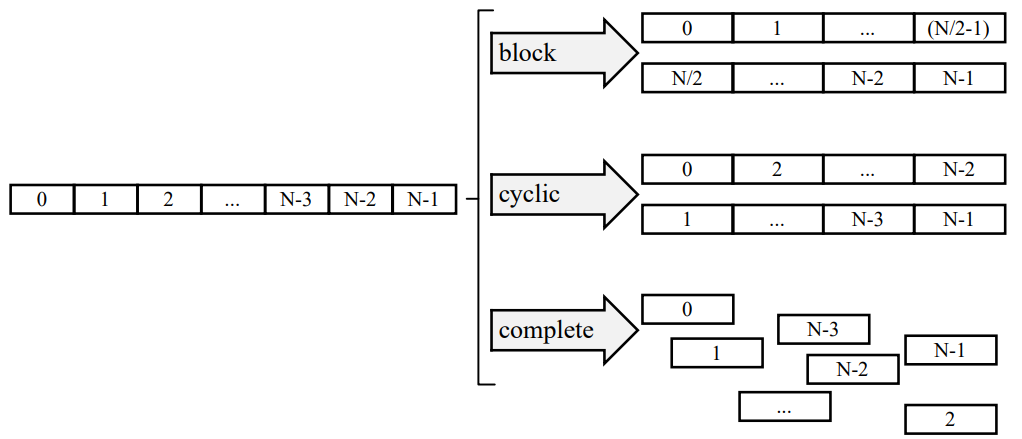
\includegraphics[width=1\textwidth]{introduction/partitioning.png}
	\caption{HLS Array Partitioning}
\end{figure}